%%% Sekce - Aplikovaná psychologie na UI/UX
%%%%% Wording: ✅
%%%%% Styling: ✅
%%%%% References: ✅
%%% --------------------------------------------------------------
\section{Aplikovaná psychologie na UI/UX}
\label{sec:navrh-uzivatelskeho-rozhrani-psychologie}

\setlength\epigraphwidth{0.8\textwidth}
\epigraph{\textit{Some people say, ``Give the customers what they want.`` But that's not my approach. Our job is to figure out what they're going to want before they do.}}{-- Steve Jobs}

Citát od Steva Jobse, zakladatele společnosti Apple, je výstižným popisem toho, co je cílem návrhu \ac{ui}.
Návrháři \ac{ui} se snaží vytvořit takové rozhraní produktu, které bude uživatelům vyhovovat a bude je bavit používat.
Aby tohoto mohlo být docíleno, je nejprve nutné aby produkt splňoval základní požadavky, jako je například funkčnost, stabilita a bezpečnost – musí splňovat nějakou minimální potřebu, jinak na ničem dalším nebude záležet\cite{bradley_hierarchy_of_needs}.

Velmi důležitým aspektem návrhu uživatelského rozhraní produktu je psychologie koncového uživatele a jeho pochopení, pro které lze využít různé psychologické teorie a koncepty jako například \textit{Maslowovu hierarchii potřeb}.
Tato hierarchie, obvykle vizualizovaná jako pyramidová struktura, ilustruje cestu jednotlivce k seberealizaci a naplnění, začínající od základních fyziologických potřeb až po složitější emoční a psychologické potřeby\cite{maslow_motivace_osobnost}.

%%% Podsekce - Maslowova hierarchie potřeb
%%%%% Wording: ✅
%%%%% Styling: ✅
%%%%% References: ✅
%%% --------------------------------------------------------------
\begin{subsection}{Maslowova hierarchie potřeb}
    \label{subsec:navrh-uzivatelskeho-rozhrani-psychologie-maslow}
    \textit{Maslowova hierarchie potřeb} je teorie psychologa Abrahama Maslowa, která se snaží definovat lidské potřeby, jejich hierarchii a vliv na lidské chování.
    Maslow tvrdil, že lidé mají potřeby, které se snaží uspokojit, ale některé z nich jsou naléhavější než jiné.
    Když jsou tyto potřeby uspokojeny, lidé se mohou cítit šťastnější, ale když nejsou, lidé mohou být frustrovaní a nespokojení.\cite{maslow_motivace_osobnost}
    Maslow rozdělil lidské potřeby do pěti základních úrovní, které jsou znázorněny na obrázku~\ref{fig:maslow} níže.

    \begin{figure}[H]
        \centering
        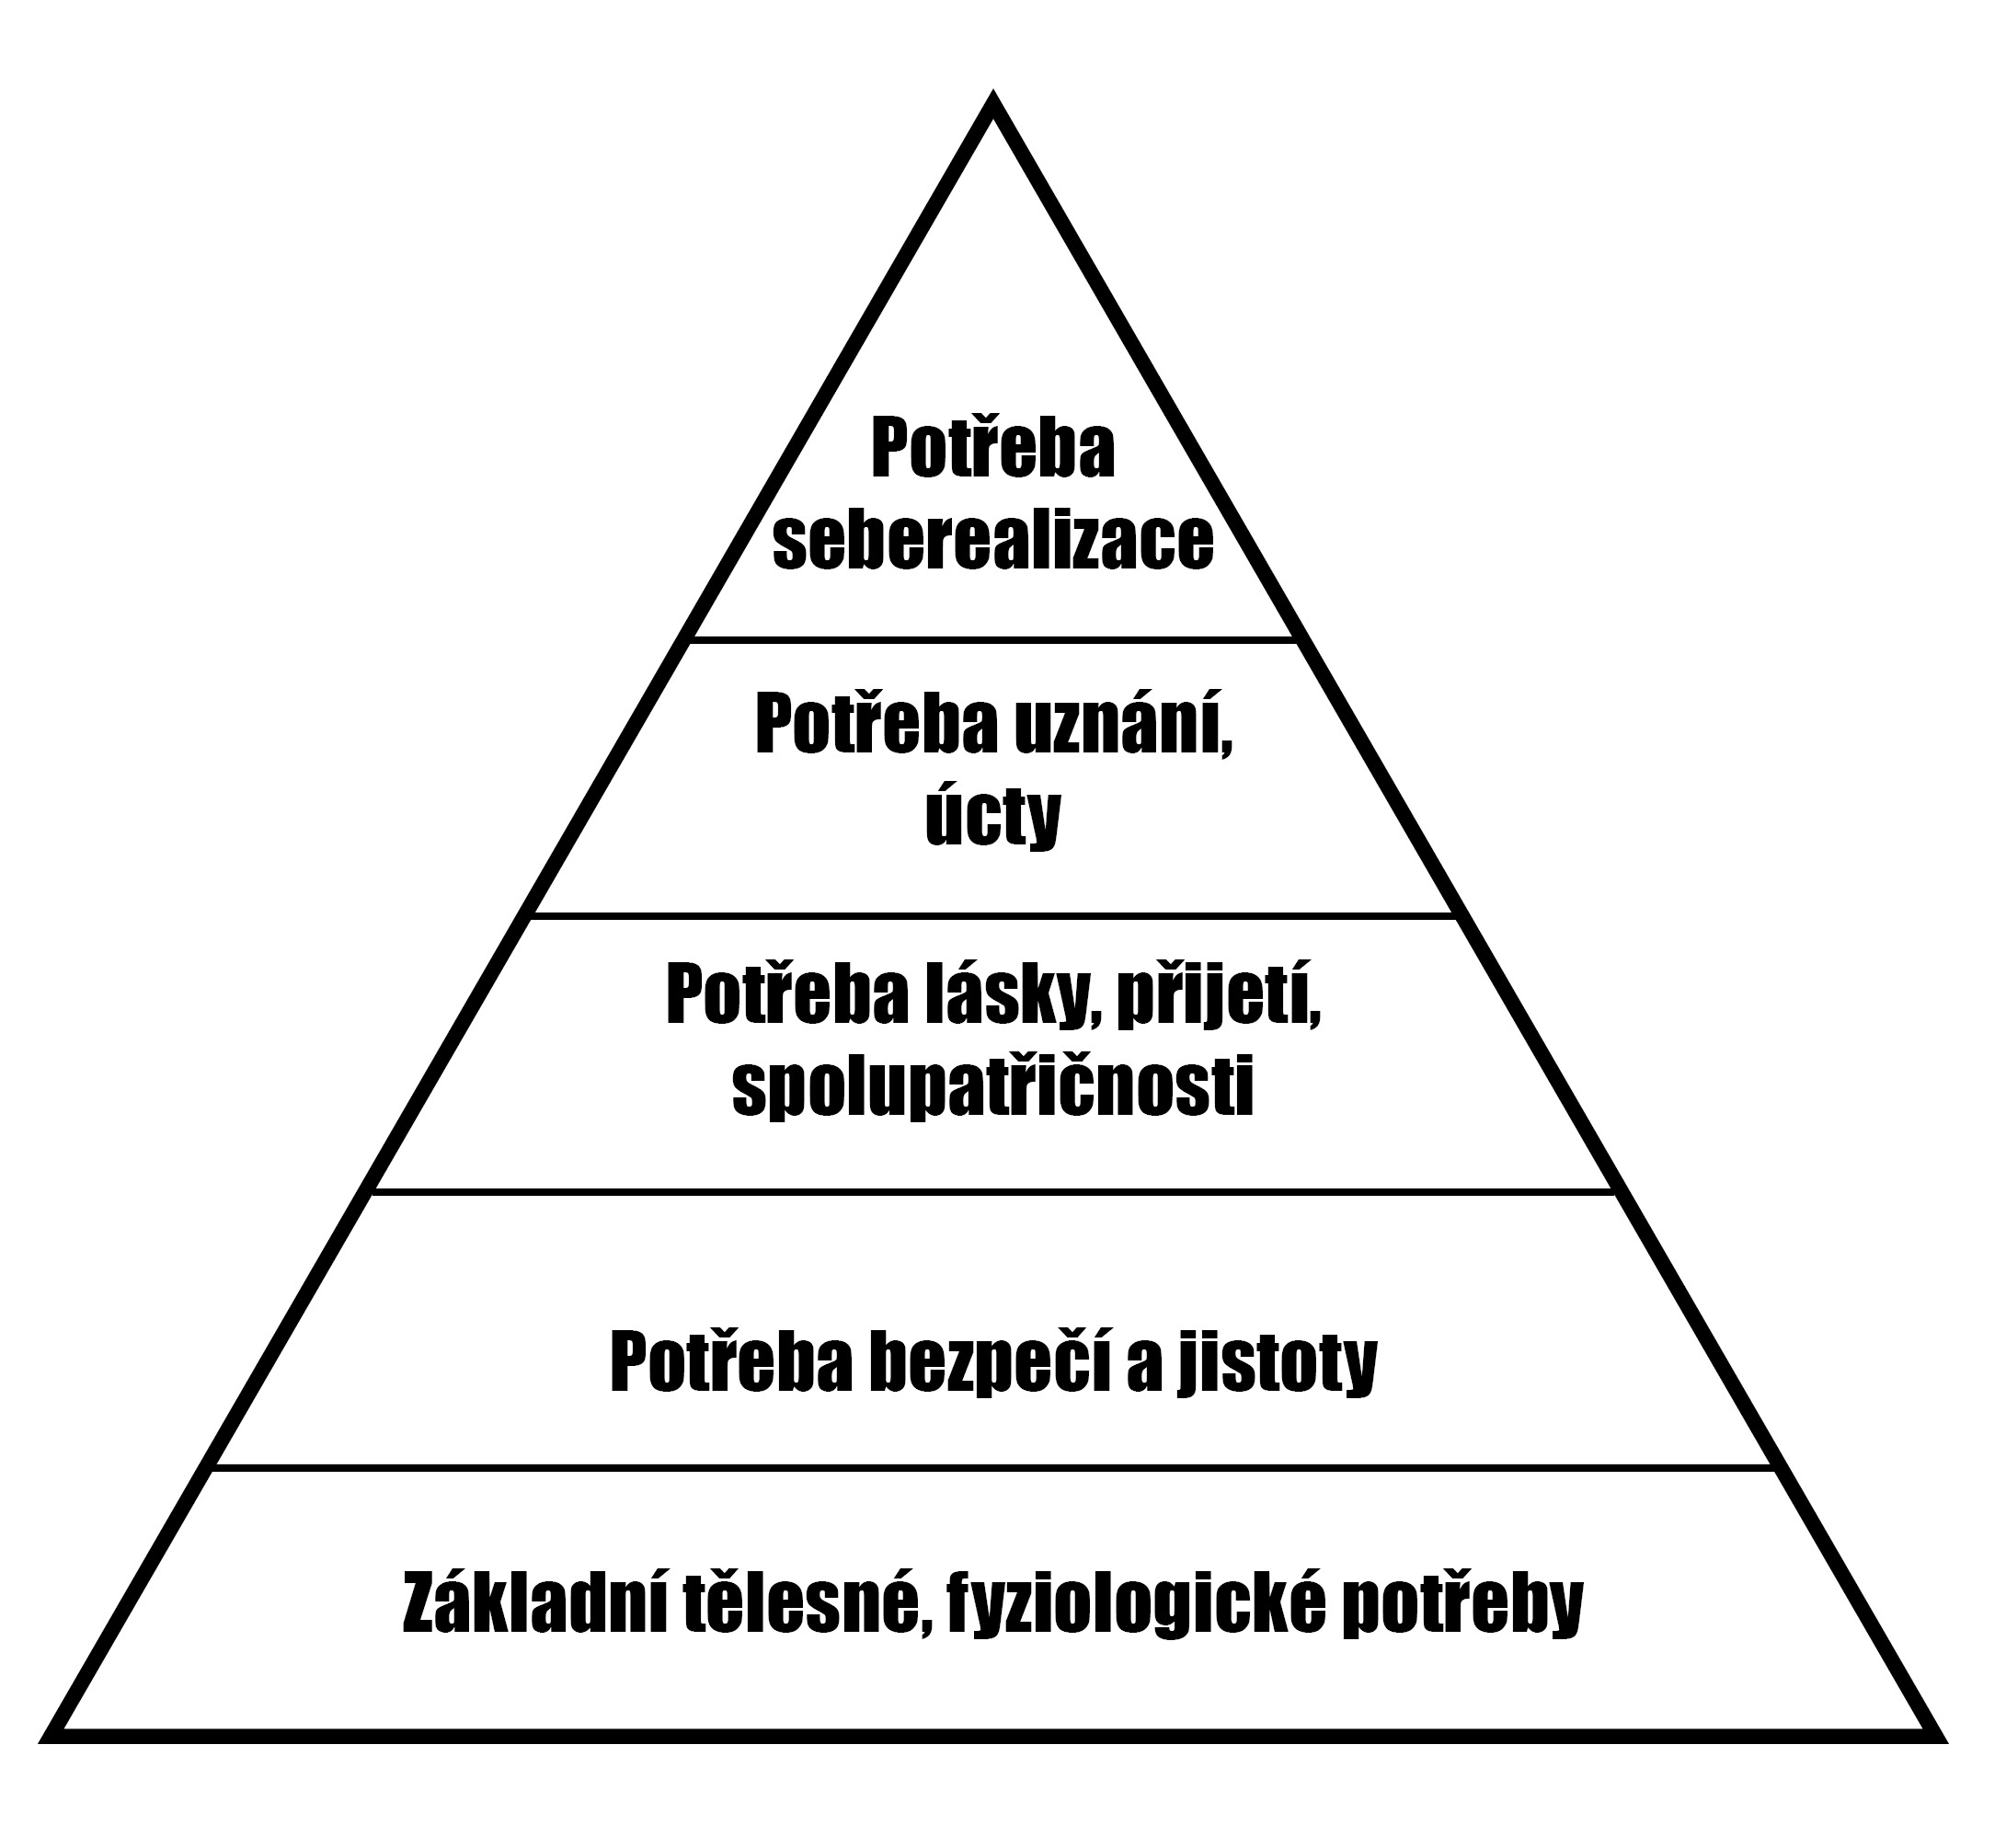
\includegraphics[width=0.8\textwidth]{\FIGDIR/maslow}
        \caption{Maslowova hierarchie potřeb\cite{wiki_potreby}}
        \label{fig:maslow}
    \end{figure}

    \begin{enumerate}
        \item \textbf{Fyziologické potřeby}: základní potřeby pro přežití, jako je potrava, voda, teplo a spánek
        \item \textbf{Potřeby bezpečí}: potřeby, které se týkají bezpečnosti a zabezpečení
        \item \textbf{Sociální potřeby}: potřeby, které se týkají příslušnosti, lásky a přátelství
        \item \textbf{Potřeby uznání}: potřeby, které se týkají úcty a sebeúcty
        \item \textbf{Potřeby seberealizace}: potřeby, které se týkají osobního růstu a rozvoje
    \end{enumerate}

    Jak to tedy ale souvisí s návrhem \ac{ui} a zejména s návrhem aplikace pro prodej vstupenek?
\end{subsection}

%%% Podsekce - Hierarchie potřeb v návrhu uživatelského rozhraní
%%%%% Wording: ✅
%%%%% Styling: ✅
%%%%% References: ✅
%%% --------------------------------------------------------------
\begin{subsection}{Hierarchie potřeb v návrhu uživatelského rozhraní}
    \label{subsec:navrh-uzivatelskeho-rozhrani-psychologie-hierarchie}
    \textbf{Maslowova hierarchie potřeb} může být aplikována na návrh \ac{ui} tak, že každá úroveň hierarchie představuje jeden základní aspekt návrhu \ac{ui}.

    V roce 2010 navrhl Steven Bradley v článku \textit{Designing For A Hierarchy Of Needs} podobnou hierarchii specificky pro design, se pěti odpovídajícími úrovněmi znázorněnými na obrázku~\ref{fig:design-hierarchy-of-needs}.\cite{bradley_hierarchy_of_needs}

    \begin{figure}[H]
        \centering
        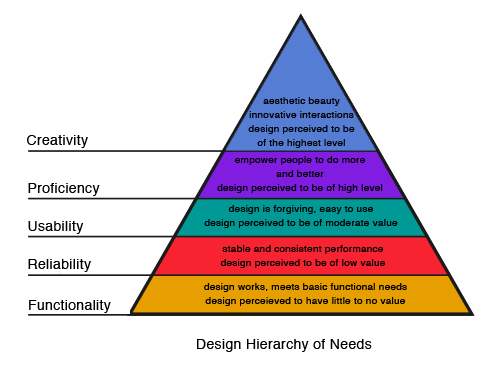
\includegraphics[width=0.8\textwidth]{\FIGDIR/design-hierarchy-of-needs}
        \caption{Hierarchie potřeb v návrhu \ac{ui} dle Stevena Bradleyho\cite{bradley_hierarchy_of_needs}}
        \label{fig:design-hierarchy-of-needs}
    \end{figure}

    \textbf{Funkčnost}\\
    Na základě pyramidy jsou základní fyziologické potřeby.
    V kontextu návrhu \ac{ui} to znamená základní funkčnost.
    Aplikace musí fungovat tak, jak se očekává, aby si uživatelé mohli vybrat sedadlo, přidat vstupenku do košíku a dokončit proces objednávky bez jakýchkoli problémů.
    Základní funkčnost musí být spolehlivá a robustní.

    \textbf{Spolehlivost}\\
    Další úroveň pyramidy je bezpečnost, která se v návrhu \ac{ui} týká spolehlivosti.
    Rozhraní by mělo být navrženo tak, aby se uživatelé cítili bezpečně a sebevědomě při interakci s ním.
    Poskytování jasných pokynů, okamžité zpětné vazby a potvrzení o úspěšných akcích (například přidání vstupenky do košíku) přispívá k pocitu bezpečí a použitelnosti.

    \textbf{Použitelnost}\\
    Střední část pyramidy pokrývá sociální potřeby, které se v \ac{ui} termínech rovnají uživatelské spokojenosti.
    Esteticky příjemné rozhraní, personalizovaný uživatelský zážitek a interaktivní prvky (jako interaktivní plán sedadel) mohou významně zvýšit uživatelskou spokojenost.

    \textbf{Odbornost}\\
    Potřeby sebeúcty zahrnují touhu po uznání a respektu.
    V kontextu aplikace pro prodej vstupenek by to mohlo znamenat přidání funkcí, které překračují očekávání uživatelů a zpříjemňují jim zážitek.
    Může se jednat o něco tak jednoduchého, jako je blahopřání po úspěšném nákupu, nebo vizuální animace při výběru sedadla.

    \textbf{Kreativita}\\
    Na vrcholu pyramidy se nachází seberealizace, která se týká realizace osobního potenciálu a hledání osobního růstu a vrcholných zážitků.
    Uživatelské rozhraní by mohlo přispět k této potřebě tím, že uživatelům umožní kreativně řešit problémy a dosáhnout svých cílů.
    Například nabízení návrhů na nejlepší dostupná sedadla nebo podobných akcí může uživatele posílit a zlepšit jejich zážitek.

    Použití Maslowovy hierarchie pro návrh \ac{ui} aplikace pro prodej vstupenek může pomoci zajistit, aby návrh splňoval potřeby uživatelů na různých úrovních.
    Z počátku je nutné zajistit základní funkčnosti a spolehlivost, aby uživatelé mohli využívat aplikaci bez jakýchkoli problémů.
    Dále je nutné zaměřit se na použitelnost, aby byl proces výběru sedadla a nákupu vstupenky co nejvíce zjednodušen.
    Při postupu v hierarchii se budou zkoumat různé metody, jak zvýšit uživatelskou spokojenost a zlepšit jejich zážitek.
    Cílem na vrcholu tohoto procesu je navrhnout rozhraní, které vyvažuje praktičnost a uživatelskou přívětivost, zatímco zároveň zajišťuje vizuální přitažlivost a emoční zapojení, což povede k přínosnějšímu, uspokojivějšímu a úspěšnějšímu uživatelskému zážitku.

    V předchozích částech byly prozkoumány základní principy návrhu uživatelského rozhraní (\ac{ui}).
    Významná část tohoto průzkumu se soustředila na to, jak lze Maslowovu hierarchii potřeb použít v návrhu uživatelského rozhraní, což slouží jako cenný rámec pro vytváření intuitivní aplikace zaměřené na uživatele.
    Zvolený způsob designu, zaměřený na fyziologické potřeby uživatele až po seberealizaci, zajišťuje, že aplikace slouží nejen svému funkčnímu účelu, ale také vytváří pro uživatele poutavý a uspokojující zážitek.

    Kromě návrhu esteticky příjemného rozhraní je důležité vytvořit systém, který skutečně vyhovuje potřebám uživatelů.
    Konečným cílem je poskytnout uživatelům intuitivní, bezproblémový a příjemný zážitek při navigaci v aplikaci, výběru sedadel a nákupu vstupenek.
    Aby tohoto mohlo být dosaženo, se následující kapitola ponoří do efektivního nástroje v designu \ac{ui}/\ac{ux} známého jako \foreign{Uživatelské příběhy}.
\end{subsection}
